\chapter{The \acl{CMS} Experiment at the \acl{LHC}}
\label{sec:experiment}
\section{Introduction}
The \acf{LHC}~\cite{lhc_design_report} is a proton-proton ($\Pp\Pp$) accelerator
located at the CERN particle physics laboratory near Geneva, Switzerland. It has
been designed to carry out a broad program of physics research using a number of
specialised detectors. This chapter will give a very brief introduction to the
\ac{LHC} itself. The \acf{CMS} experiment, a large, general purpose detector at
the \ac{LHC}, will be discussed in detail.

\section{The \acl{LHC}}
The \ac{LHC} is a circular synchrotron, \unit{27}{\kilo\metre} in circumference,
sitting on the border between France and Switzerland. It has been built in a
tunnel initially constructed to house the \ac{LEP} accelerator, buried at a
depth of between 50 and \unit{175}{\metre} underground. Although primarily a
$\Pp\Pp$ accelerator, the \ac{LHC} will also undertake a heavy-ion physics
program. At full design specifications, 2808 bunches of protons will circulate
around each direction of the ring, colliding at a centre-of-mass energy of
\unit{14}{\TeV}. It is designed to eventually reach a proton bunch spacing of
\unit{25}{\ns} and an instantaneous luminosity of
\unit{$10^{34}$}{\rpsquare{\centi\metre}\usk\reciprocal\second}.

There are four primary experiments at the \ac{LHC}:
\ac{ALICE}~\cite{alice_proposal}, \ac{ATLAS}~\cite{atlas_proposal},
\ac{CMS}~\cite{cms_technical_proposal,cms_jinst} and the
\ac{LHCb}~\cite{lhcb_proposal} experiment. Each one is constructed around one of
the four interaction points and records the shower of particles produced from
the colliding protons. \ac{ATLAS} and \ac{CMS} are large, general purpose
detectors, designed to search for a variety of \ac{NP} signatures as well as
making higher precision measurements of many \ac{SM} parameters. \ac{ALICE} is
optimised to examine the products of heavy-ion collisions (principally lead-lead
-- although a number of configurations are possible) in order to explore the
quark-gluon plasma and related physics. Finally, the \ac{LHCb} experiment is
optimised for the study of B-meson decays. These are important for the study of
CP violation within the \ac{SM} but might also provide potential avenues for the
discovery of \ac{NP}.

In addition to the four larger detectors, two smaller experiments lie upstream
of the \ac{ATLAS} and \ac{CMS} collision points in order to probe more
specialised forward physics phenomena. These are the
\ac{LHCf}~\cite{lhcf_proposal} and \ac{TOTEM}~\cite{totem_proposal} experiments.

\subsection{Accelerator Complex}
The \ac{LHC} ring itself is the final stage in an injector chain which
incorporates a series of accelerators built at CERN over the last 50 years. It
is illustrated in \fig~\ref{fig:expt_lhc}. Each stage supplies an incremental
increase in the proton (or heavy ion) bunch energy. The first stage in this
chain is a linear accelerator -- either the Linac2 for proton injection or
Linac3 during heavy-ion runs. The Linac2 injects protons into the \ac{PSB} at an
energy of \unit{50}{\mega\electronvolt}. Similarly, the ions proceed first from
the Linac3 to the \ac{LEIR} before finally arriving at the \ac{PS}. From here
on, the paths of the protons and heavy-ions are the same. Proton bunches pass
from the \ac{PSB} to the \ac{PS} at an energy of \unit{1.4}{\giga\electronvolt}
and then on to the \ac{SPS} at an energy of
\unit{26}{\giga\electronvolt}. Having arrived at the \ac{SPS}, the protons (or
heavy-ions) circulate around a ring \unit{2}{\kilo\metre} in diameter, where
their energy is increased to \unit{450}{\giga\electronvolt}. From here, kicker
magnets inject the bunches into the \ac{LHC} itself, where the energy can
finally be increased to the design-specified \unit{7}{\TeV} per beam. The 2010
and 2011 data-taking periods were at \unit{3.5}{\TeV} per beam, with an increase
to \unit{4}{\TeV} planned for 2012.

\begin{figure}[h!]
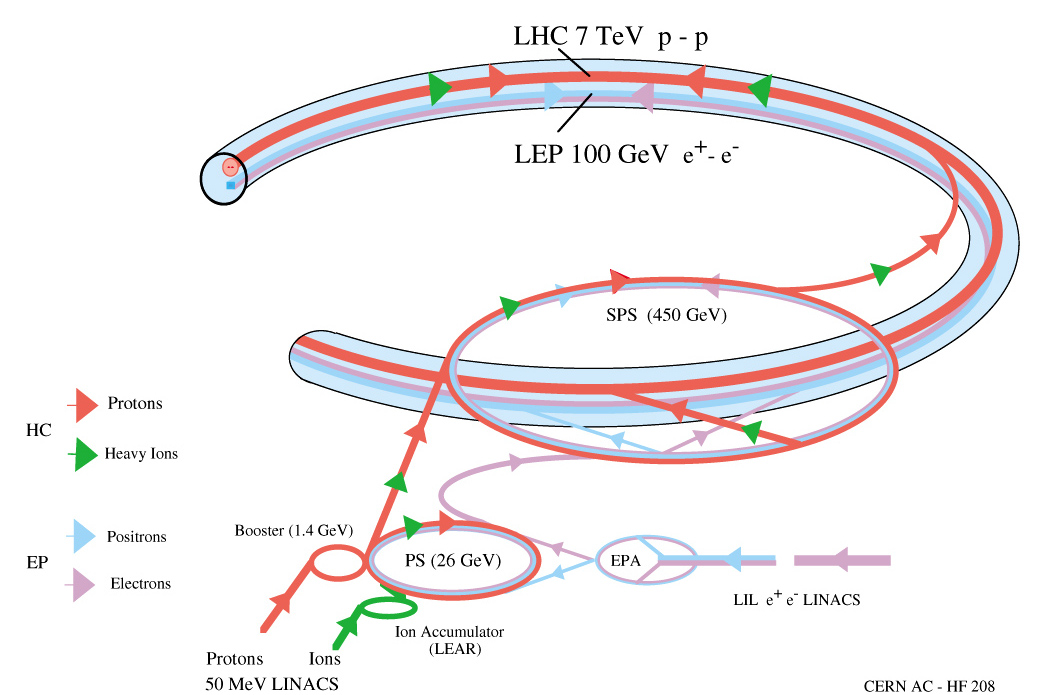
\includegraphics[width=0.8\textwidth]{fig/lhc-pho-1993-008_cropped}
\caption[Illustration of the \acs{LHC} accelerator complex]{Illustration of the
  \ac{LHC} accelerator complex showing the path of protons and heavy-ions
  through a series of accelerators at \ac{CERN}~\cite{lhc_injection}.}
\label{fig:expt_lhc}
\end{figure}

\section{The \acl{CMS} Experiment}
\label{sec:cms}
\ac{CMS} is a large, general purpose detector~\cite{cms_jinst} at the
\ac{LHC}. It has been designed to search for the Higgs boson (see
\sec~\ref{sec:sm_higgs}) as well as signatures of physics beyond the \ac{SM}.

The design goals of CMS were as follows (paraphrasing the technical proposal
document~\cite{cms_technical_proposal}):
\begin{enumerate}
\item a high quality, redundant muon system,
\item the best possible \ac{ECAL}
\item high quality central tracking to complement these two systems and
\item an affordable detector.
\end{enumerate}

\begin{figure}[h!]
\centering
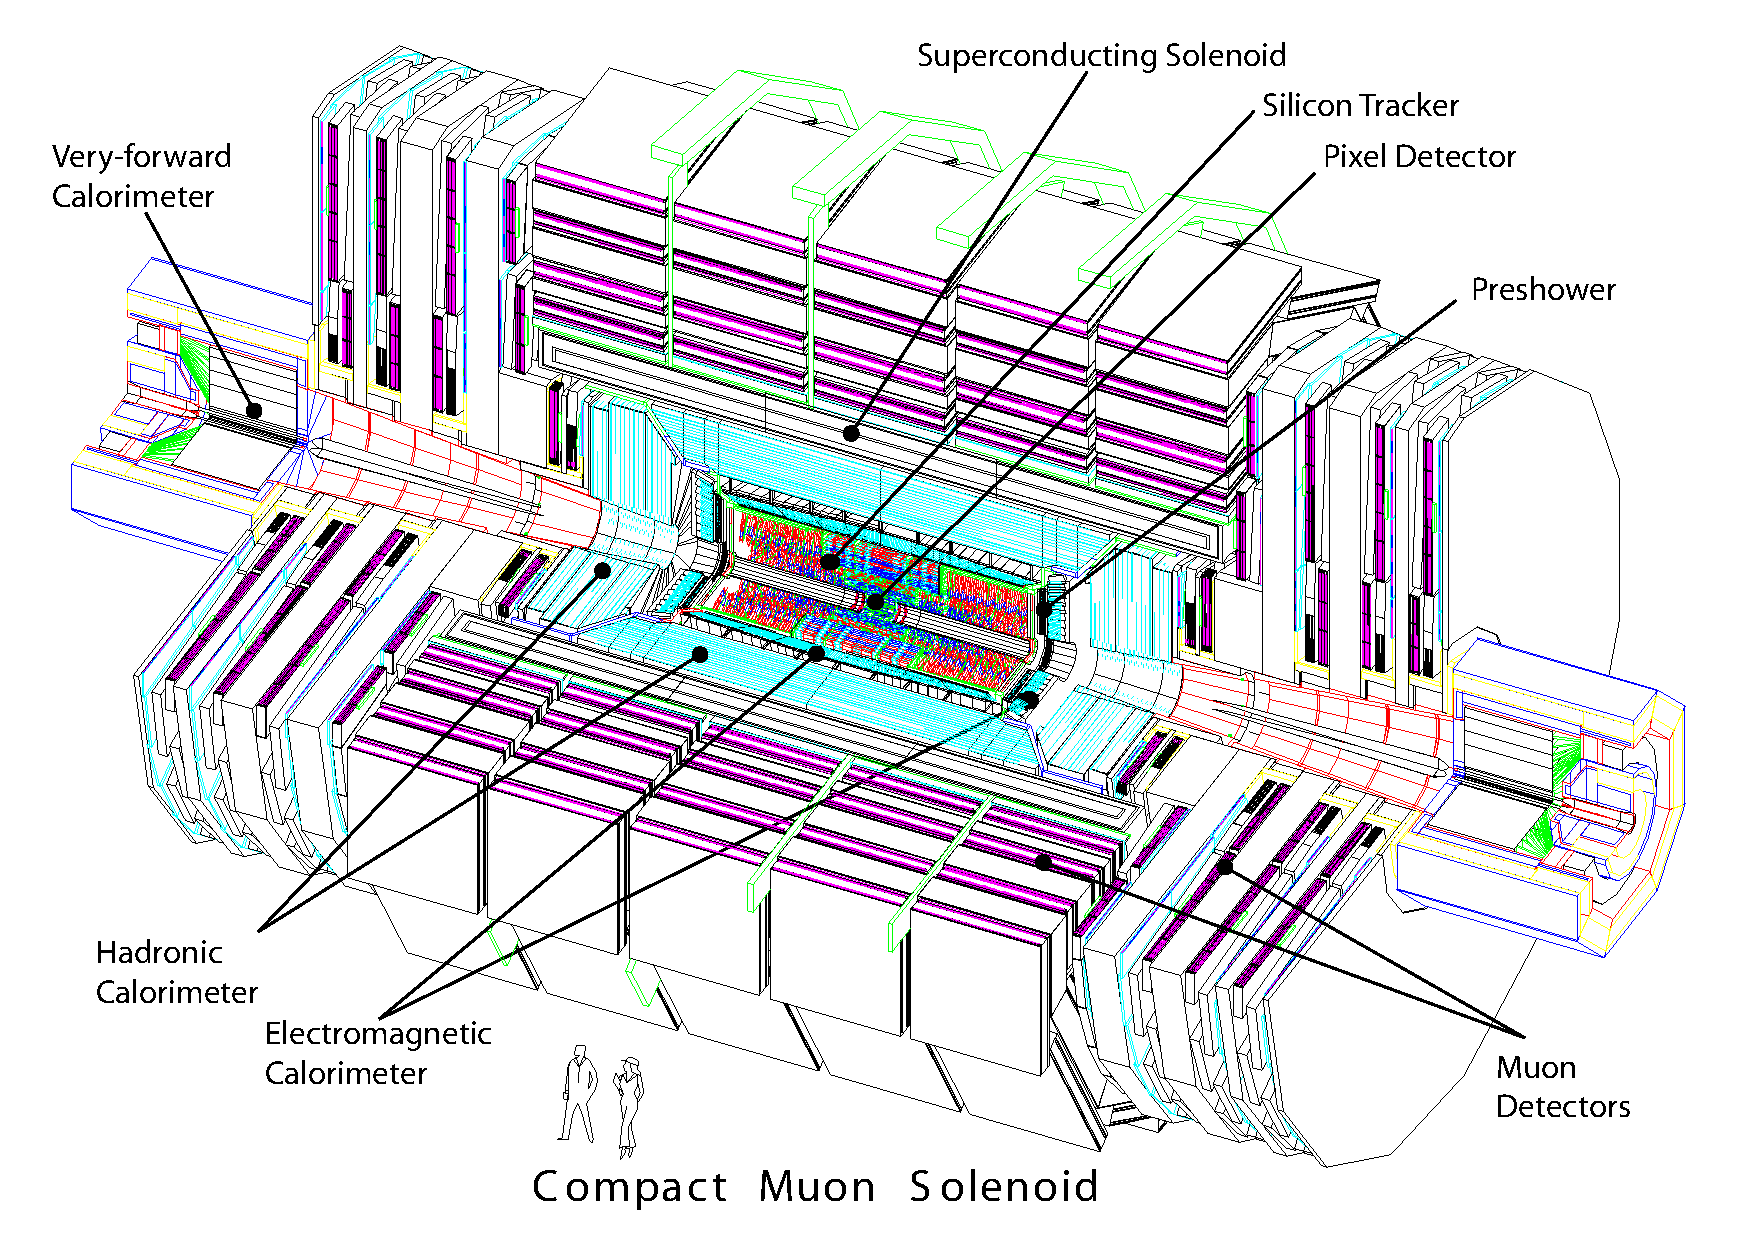
\includegraphics[width=0.7\textwidth]{fig/cms_complete_labelled}
\caption[Illustration of the \acs{CMS} detector]{Illustration of the \ac{CMS}
  detector with subdetectors labelled~\cite{cms_jinst}.}
\label{fig:expt_cms}
\end{figure}

\ac{CMS} adopts a traditional cylindrical design (see
\fig~\ref{fig:expt_cms}), \unit{21.5}{\metre} in length and \unit{15}{\metre}
in diameter. A key feature of the detector is the \unit{4}{\tesla}
superconducting solenoid. The bending field supplied provides accurate muon
momentum resolution up to energies of \unit{$\approx$ 1}{\TeV}. The size of the
solenoid placed stringent limitations on the volume of the inner detector
subsystems (everything except for the muon chambers and return yoke).

\subsection{Coordinate System}
The coordinate system at \ac{CMS} is right-handed, with its origin placed at the
nominal beam collision point inside \ac{CMS}. The $x$ axis is then defined to
point horizontally inwards towards the centre of the \ac{LHC} ring and the
$y$-axis, vertically upwards. The $z$-axis is aligned along the beam-line,
pointing towards the nearby Jura mountains. Often a cylindrical coordinate
system will be used where the azimuthal angle, $\phi$, and radial
coordinate, $r$, span the $x-y$ plane. The azimuthal angle is measured with
respect to the $x$-axis. The pseudorapidity, $\eta = - \ln \tan
\frac{\theta}{2}$ where $\theta$ is the polar angle measured with respect to the
$z$-axis.

\subsection{Silicon Tracker}
The innermost subsystem of \ac{CMS} is the silicon tracker~\cite{tracker_paper},
designed to provide highly precise measurements of particle trajectories close
to the CMS interaction point. It is shown in cross section in
\fig~\ref{fig:expt_tracker}. The tracker extends to pseudorapidities of
$|\eta|<2.5$ and has an active silicon area of more than
\unit{200}{\metre\squared}, making it the largest silicon tracker ever built.

\begin{figure}[h!]
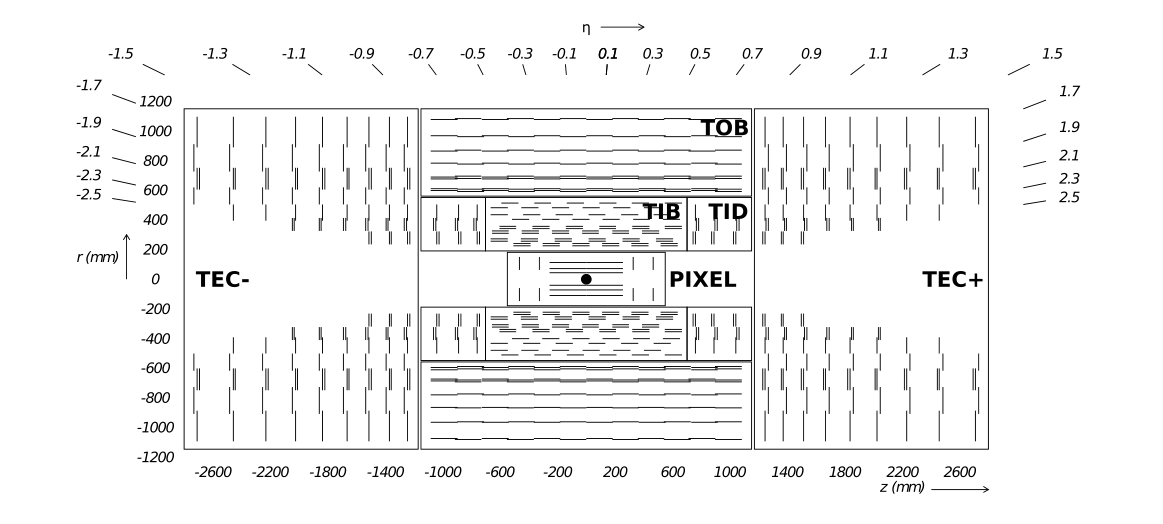
\includegraphics[width=\textwidth]{fig/tracker2}
\caption[Schematic cross section through the CMS tracker]{Schematic cross
  section through the CMS tracker. Each line represents a detector
  module. Double lines indicate back-to-back modules which deliver stereo
  hits~\cite{cms_jinst}.}
\label{fig:expt_tracker}
\end{figure}

The tracker design can be better understood by considering the expected particle
flux at design luminosity as a function of radial distance, $r$, from the
beam-line.
\begin{itemize}
\item At $ r \approx \unit{10}{\cm}$ the particle flux is highest. Accordingly,
  the innermost layer of the CMS tracker is comprised of hybrid pixels. With an
  area of \unit{$100\times 150$}{\micro\metre\squared}, particle densities are
  $O(10^{-4})$ per pixel per LHC bunch crossing.
\item At a radius \unit{$20 < r < 55$}{\centi\metre}, reduced particle flux allows
  the use of silicon microstrip sensors. With a much larger area of
  $\unit{10}{\centi\metre}\times\unit{80}{\micro\metre}$, average particle
  densities are $O(10^{-2})$ per strip per bunch crossing.
\item At $ r > \unit{55}{\cm}$, still larger silicon strips can be used, with
  sizes up to $\unit{25}{\cm}\times\unit{180}{\micro\metre}$. This gives a
  particle density of $O(10^{-2})$ per strip per bunch crossing.
\end{itemize}

\subsubsection{Pixel Tracker}
The hybrid pixels are placed closest to the interaction point. As well as
maintaining an acceptable particle density per sensor, their close proximity to
the interaction point allows the origin of collision products to be accurately
determined. In the barrel region, 3 layers are placed at mean radii of 4.4, 7.3
and \unit{10.2}{\cm}. The detector has a length of \unit{53}{\cm} in the $z$
direction. The end discs are instrumented with only two layers and are located
at $|z|=34.5, \unit{46.5}{\cm}$. The pixel modules in these layers are arranged
in a ``turbine-like'' layout.

\subsubsection{Strip Tracker}
Further from the interaction point, the tracker is instrumented with silicon
strip detectors. The barrel component can be further divided into the \ac{TIB}
and the \ac{TOB}. The \ac{TIB} is composed of 4 layers and the \ac{TOB} a
further 6. The \ac{TOB} extends to $z = \pm \unit{118}{\centi\metre}$. Beyond
this are the endcaps which can again be split into two components: the \ac{TEC}
made up of 9 disks and the \ac{TID}, 3. The silicon micro-strip sensors are
\unit{320}{\micro\metre} thick and oriented parallel to the $z$-axis in the
barrel and radially in the disks.

Both the \ac{TIB} and \ac{TID} supply up to four measurements in $r\phi$. The
inner two layers of the \ac{TIB} have a strip-pitch of \unit{80}{\micro\metre},
and the outer two, \unit{120}{\micro\metre}. These achieve single point
resolutions of \unit{23 and 35}{\micro\metre} respectively. In the \ac{TID}, the
strip pitch varies between \unit{100 and 141}{\micro\metre}.

The \ac{TOB} uses \unit{500}{\micro\metre} thick sensors with a strip-pitch of
\unit{183}{\micro\metre} in the first four layers and \unit{122}{\micro\metre} in
the outer two. This gives a single point resolution of \unit{53}{\micro\metre}
and \unit{35}{\micro\metre} respectively.

The first two layers of the \ac{TIB}, \ac{TOB} and \ac{TID} and rings 1, 2 and 5
of the \ac{TEC} are so-called ``stereo modules''. These are double-sided modules
where the two layers of strips have a stereo angle of \unit{100}{\milli\radian}
between them. This provides additional resolution in the $z$ measurement in the
barrel (or $r$ in the endcaps). The resolution of this measurement is
\unit{230}{\micro\metre} and \unit{530}{\micro\metre} in the \ac{TIB} and
\ac{TOB} respectively.

\subsection{\acl{ECAL}}
The \ac{ECAL} surrounds the silicon tracker and provides a high resolution
measurement of electromagnetic showers within a homogeneous, hermetic
calorimeter~\cite{ecal_paper}. The barrel region alone comprises 61,200 lead
tungstate (PbWO$_4$) crystals, with 7,324 in each of the two endcaps. This
material was chosen for its high density, short radiation length and small
Moli\`{e}re radius. Scintillation photons are then recorded by \acp{APD} in the
barrel and \acp{VPT} in the endcap. The driving motivation for the \ac{ECAL}
design was the detection of the low-mass favoured Higgs decay channel
$\PH\longrightarrow\gamma\gamma$.

\subsubsection{\acl{EB}}
The \ac{EB} extends in rapidity to $|\eta|<1.479|$ with a crystal segmentation
of $360\times 85$ in $\eta-\phi$ for each half-barrel. Each crystal is slightly
tapered, with a cross-section of $0.0174\times0.0174$ in $\eta-\phi$. The
crystals have a front cross section of \unit{$22\times
  22$}{\milli\metre\squared} and a length of \unit{230}{\milli\metre}
(corresponding to 25.8 radiation lengths).

\subsubsection{\acl{EE}}
The \ac{EE} occupies the rapidity range $1.479 < |\eta| < 3.0$. Crystals are
grouped into $5\times 5$ ``supercrystals'' within a carbon-fibre alveolar
structure. The endcaps are split into two halves, known as ``Dees'', each
holding 3,662 crystals.

The scintillation of the \ac{ECAL} crystals as well as the amplification of the
\acp{APD} varies as a function of temperature. This variation was found to be
\unit{$\approx 4\%$}{\per\celsius}. For this reason, the \ac{ECAL} temperature
is precisely regulated to within \unit{$\pm$ 0.05}{\celsius}.

\subsubsection{\ac{ECAL} Transparency and the \ac{CMS} Laser Monitoring System}
\label{sec:expt_laser_monitoring}
The PbWO$_4$ crystals that make up the \ac{ECAL} are radiation resistant but
quickly suffer a decrease in their optical transmission under
irradiation~\cite{ecal_transparency}. This is a result of the formation of
colour centres which absorb a fraction of the incident light. At a working
temperature of \unit{18}{\celsius}, the damage anneals leading to an equilibrium
in the optical transmission properties -- constant with dose rate. The
consequence of this is a cyclic change in the optical transmission rate of the
crystals as the \ac{LHC} moves between colliding beams and machine
refills. Since this depends on dose rate, the effect is a function of \ac{LHC}
luminosity and rapidity. It is expected to range from a shift of $\sim 2\%$ in
the barrel at low luminosity to $> 10\%$ in the endcaps at high luminosity. The
magnitude of this effect on energy and momentum measurements would be disastrous
if not properly accounted for. Correction for this effect necessitates constant
monitoring of the transparency -- a task performed by the laser monitoring
subsystem~\cite{laser_monitoring}.

Three lasers are used for the transparency measurement: two blue ($\lambda
\approx \unit{440}{\nano\metre}$) and one near-infrared ($\lambda \approx
\unit{796}{\nano\metre}$). The blue laser (with a second fitted for redundancy
purposes) is close to the scintillation emission peak and thus can be used to
track the changes in the crystal transparency. The near-infrared laser is far
from the emission peak and thus relatively stable to changes in the
transparency. This can be used to verify the stability of the system. The lasers
are distributed to the crystals via optical fibres and a series of
fan-outs. Approximately 1\% of the \ac{LHC} beam gap of
\unit{3.17}{\micro\second} is used for transparency monitoring. A full scan of
the entire \ac{ECAL} can be achieved in approximately 30~minutes. The lasers can
be pulsed at $\approx \unit{80}{\mega\hertz}$ with a pulse timing jitter of
\unit{3}{\nano\second}. This is adequate for synchronisation with the \ac{LHC}
bunch crossings.

The transparency of the crystals is derived from the response of the \ac{APD}
normalised to the height of the laser pulse, as measured using a silicon
photodiode. Due to differences in path length and optical spectra between the
laser and the scintillation light, the transparency of the crystals may be
related to the measured transparency via a power law.

\subsection{\acl{HCAL}}
Accurate measurement of hadronic showers is crucial for analyses involving jets
or missing energy signatures. The \ac{HCAL}~\cite{hcal_paper} lies between the
outer edge of the ECAL and the inner edge of the solenoid ($\unit{1.77}{\metre}
< r < \unit{2.95}{\metre}$). This constrains the size of the \ac{HCAL} to a
relatively compact design and necessitates the placement of a ``tail catcher''
outside of the solenoid.

\subsubsection{\acl{HB}}
The \ac{HB} comprises 36 azimuthal wedges, with 18 in each half barrel. Each
wedge consists of alternating layers of brass absorber plates and plastic
scintillators. The light from these plates is then carried via
wavelength-shifting fibres to a \ac{HPD} for readout. The number of interaction
lengths increases with polar angle, from 5.82 at $90\degrees$ to 10.6 at
$|\eta|=1.3$~\cite{hcal_design}.

\subsubsection{\acl{HE}}
The \ac{HE} covers the rapidity range $1.3 < |\eta| < 3$ and receives a larger
radiation flux than the \ac{HB}. Each endcap consists of 36 wedges, and
wavelength shifting fibres are once again used to take light from plastic
scintillators to \acp{HPD}. Including the \ac{ECAL}, the \ac{HE} depth is
equivalent to $\approx 10$ interaction lengths.

\subsubsection{\acl{HO}}
The \ac{HO} or ``tail catcher'' provides increased sampling depth in the
rapidity region $|\eta| < 1.3$ where the \ac{HB} and \ac{EB} do not provide
sufficient containment. Since the \ac{HO} lies outside the solenoid, its design
is constrained by that of the muon chambers -- with 5 rings in $\eta$. The
solenoid coil provides additional absorption, giving the calorimeter system a
minimum depth of 11.6 interaction lengths.

\subsubsection{\acl{HF}}
The \ac{HF} is positioned in the rapidity range $|\eta|>3$ and consequently must
endure a much larger particle flux -- approximately \unit{760}{\GeV} per
proton-proton interaction (versus $\approx \unit{100}{\GeV}$ for the rest of the
detector). Radiation hardness was thus a leading consideration in its design.

Quartz fibres are interleaved between steel absorbers. Shower particles above
the Cherenkov threshold ($E \geq \unit{190}{\keV}$ for electrons) produce
Cherenkov light. This is routed to the rear of the calorimeter and read out by
\acp{PMT}. The \ac{HF} is most sensitive to the electromagnetic component of the
shower.

\subsection{Muon Chambers}
Accurate measurement of muons is one of \ac{CMS}'s key design goals. The effect
of radiative losses in the tracker is much less for muons than it is for
electrons. Thus muons are able to provide a much finer mass resolution at low
transverse momentum. This is an important advantage for a variety of physics
searches and measurements at \ac{CMS}. The muon system is responsible for muon
identification, momentum measurement and triggering (for further detail see
\sec~\ref{sec:trigger}). Three types of detectors are used, chosen for different
regions of the detector according to the magnetic field, muon rate and response
time required for input to the trigger.

\subsubsection{\aclp{DT}}
In the barrel region, the magnetic field is relatively uniform and the muon flux
low enough to allow the use of the \acf{DT}~\cite{dt_paper}. These identify
muons in the region $|\eta| < 1.2$. The drift chamber was first developed as a
refinement of earlier wire proportional chamber designs in which the drift time
of the electrons to the anode wire is used to provide additional spatial
resolution. This allows the wire spacing to be increased, thus reducing the
electronics requirements.

Each \ac{DT} is composed of 2 (or 3) ``super-layers'', with each super-layer
further divided into 4 layers of rectangular drift cells. Of the four concentric
muon stations in the barrel, the inner three contain 60 drift chambers and the
outermost, 70. The wires in the outer two layers of each drift cell are oriented
parallel to the beam line, providing a measurement in the $r\phi$ direction (the
magnetic bending plane). The inner two layers are perpendicularly aligned,
giving a measurement of the $z$ coordinate.

\subsubsection{\aclp{CSC}}
In the endcap region, the large muon and background rate coupled with the
strong, non-uniform magnetic field, prevent the use of \acp{DT}. Instead, an
alternative instrument is used -- the \ac{CSC}~\cite{csc_paper}. The CMS muon
system endcap consists of 468 \acp{CSC}, each a trapezoidal multiwire
proportional chamber arranged radially covering an azimuthal angle $\Delta\phi$
of either 10 or 20 degrees. Each \ac{CSC} is a multiwire proportional chamber
with 6 anode wire planes interleaved with 7 cathode strip planes. The wire
readout provides a measurement of the $\phi$ coordinate whilst a measurement of
$r$ is obtained by interpolating charges on the cathode strips.

\subsubsection{\aclp{RPC}}
The trigger (see \sec~\ref{sec:trigger}) requires a muon detector capable of
providing a fast signal with adequate spatial resolution. This is the
\acf{RPC}~\cite{rpc_paper}, a gaseous, parallel-plate detector with spatial
resolution suitable for both barrel and endcap regions and a response time much
less than the \unit{25}{\nano\second} between consecutive \ac{LHC}
bunch-crossings. This allows the \ac{RPC} to unambiguously identify the
bunch-crossing assignment for a muon track, even in the presence of the large
backgrounds and high rates of the \ac{LHC} environment.

\subsection{Data Acquisition and Trigger System}
\label{sec:trigger}
The high luminosity of the \ac{LHC} beam leads to a high particle flux in the
detector. The separation of particles in the detector becomes increasingly
difficult. In addition, many analyses benefit from precise position and momentum
measurements. Consequently, the \ac{CMS} subdetectors are constructed with an
extremely fine granularity. Unavoidably, this requires an extremely large number
of read-out channels - approximately 55 million across the whole detector. To
make matters worse, the \ac{LHC} is planned to achieve a bunch-spacing of only
\unit{25}{\nano\second}. For these reasons, the \ac{DAQ} system at \ac{CMS}
faces the simultaneous challenges of large bandwidth and low-latency.

Tightly coupled to the \ac{DAQ} is the trigger system~\cite{tridas}. The huge
number of readout channels in \ac{CMS} is not only a challenge in terms of the
bandwidth of the \ac{DAQ} but also poses serious difficulties relating to
long-term storage requirements. A digitised, zero-suppressed event dump from
\ac{CMS} is approximately \unit{2}{\mega\byte} in size. With an event rate of up
to \unit{40}{\mega\hertz}, this would require a storage rate of
\unit{80}{\tera\byte\per\second}. Despite the rapid improvement in disk storage
technology over the last few decades, such storage capacities are clearly
infeasible both in terms of capacity and \ac{IO} requirements. For these
reasons, a system capable of quickly rejecting a very large fraction of
collisions is required. This is known as the trigger.

\subsubsection{Triggering at \ac{CMS}}
The trigger at \ac{CMS} is split into two stages. The first stage, the \ac{L1T},
must operate at the full \ac{LHC} bunch-crossing frequency. To achieve adequate
latency, it is implemented almost entirely within electronic logic -- either
\acp{FPGA} or custom designed integrated circuits. The \ac{L1T} must reduce the
rate to \unit{100}{\kilo\hertz}.

In the second stage of the trigger, the \ac{HLT}, the rate is further reduced to
$O(\unit{100}{\hertz})$. Due to the reduced rate, the \ac{HLT} is implemented in
software running in a computing farm. Since the \ac{HLT} has access to a full
read-out of the detector, and more time to issue a trigger decision, more
sophisticated trigger algorithms are used. Often these are similar to those used
by the off-line reconstruction.

\subsubsection{The \acl{L1T}}
The \ac{L1T} must produce a trigger decision with minimal latency. This latency
is chiefly limited by the size of the pipeline on the \ac{APV25} chip used to
readout from the silicon strip tracker. The \ac{APV25} samples the voltage from
the silicon strips at \unit{25}{\nano\second} intervals. These are stored in a
pipeline, 192 samples deep. This constrains the \ac{L1T} to provide a decision
within $\approx \unit{3.2}{\micro\second}$.

The \ac{L1T} has limited access to detector subsystems and only a limited time
in which to issue a trigger decision. In particular, since tracker measurements
are not available, distinction between electrons and photons is not
possible. The challenge for the \ac{L1T} is therefore not only to make a fast
decision using limited information from the detector, but also to ensure that
potentially interesting events are retained and passed onto the \ac{HLT} for
more thorough analysis.

\begin{figure}[h!]
\centering
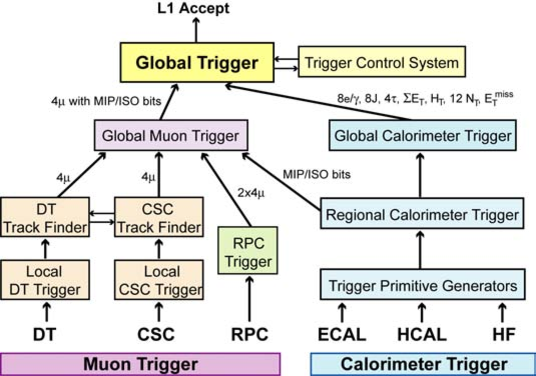
\includegraphics[width=0.7\textwidth]{fig/trigger}
\caption[Diagram showing the organisation of the \acs{CMS} \acs{L1T}]{Diagram
  showing the organisation of subsystems within the \ac{CMS} \ac{L1T}.}
\label{fig:expt_cms_trigger}
\end{figure}

The structure of the \ac{L1T} is shown in \fig~\ref{fig:expt_cms_trigger}. The
\ac{GT} is the final stage in the trigger chain. It receives ``trigger objects''
from two subsystems: the \ac{GCT} and \ac{GMT}. Objects, ranked according to
their energy and quality, are received along with their coordinates in $\eta$
and $\phi$. These objects are processed by 128 algorithms, each of which
produces a trigger decision. The final output of the \ac{GT} is then determined
by a configurable mask, which may be altered to meet different data-taking
objectives. The final trigger decision is then sent to the Timing, Trigger and
Control subsystem in order to initiate a read-out of the detector.

The calorimeter trigger subsystem begins with the \ac{TPG}. This sums energy
deposits from the \ac{ECAL} and \ac{HCAL} into ``trigger towers''. These are
received by the \ac{RCT}, where electron/photon candidates are found and the
trigger tower energies summed into larger ``\ac{RCT} regions''. These consist
of $4\times 4$ trigger towers (except in the \ac{HF} where only a single trigger
tower is included). The \ac{RCT} also records a ``tau-veto'' bit, used to
distinguish jets from hadronic tau decays.

The output of the \ac{RCT} is then processed by the
\ac{GCT}~\cite{jj_thesis}. The \ac{GCT} logic is implemented primarily in
\acp{FPGA}. The \ac{GCT} performs a number of tasks in parallel. It sorts the
list of electron/photon candidates and passes the four highest ranked objects to
the \ac{GT}. It also performs a simple jet-finding algorithm on the \ac{RCT}
regions, classifying them as \emph{forward}, \emph{central} and \emph{tau}
jets. The last category includes jets for which none of the constituent \ac{RCT}
regions has its tau-veto bit set. The four highest ranked of each category are
then forwarded to the \ac{GT}.

The final task of the \ac{GCT} is to form global energy sums. These are the
total transverse energy, missing transverse energy, jet counts and \HT (the
scalar sum of the jet energies). These too are forwarded to the \ac{GT}.

The muon trigger receives input from all three muon subdetectors: \acp{RPC},
\acp{CSC} and \acp{DT}. These are integrated in the \ac{GMT}. The muons received
from each subdetector are matched and sorted by transverse momentum and
quality. The four highest rank candidates are forwarded to the \ac{GT}.

\subsection{Computing at \acs{CMS}}
\label{sec:cms_computing}
To meet the extremely large computation and storage requirements of data analysis
at the \ac{LHC}, analysis tasks are performed using a dedicated computing
grid~\cite{lhc_grid}. Events are first sent to the ``tier-0'' storage site at
\ac{CERN} with additional copies forwarded to a number of ``tier-1'' sites
around the world. Data is made available for analysis use, in various
re-processed forms, at ``tier-2'' and ``tier-3'' grid sites. User analysis jobs
are submitted to the grid, and routed automatically to a suitable site.

Events recorded by the \ac{CMS} detector pass through a chain of reconstruction
stages. At each stage, higher-level physics objects are built out of simpler
ones, with a consequent reduction in the data size. \ac{MC} events are processed
using either a detailed \geantfour simulation~\cite{geant_paper}, or a faster,
parameterised model of the response known as \fastsim. This simulates the
response of the \ac{CMS} subdetectors to the generated particles. After the
detector response has been simulated, \ac{MC} is processed in exactly the same
manner as data.
